\section{Imaging artifacts}
\label{sec:imaging}

Noise in tomography is unavoidable, and it makes segmentation harder because it
further obscures the boundaries between materials.  Materials may be well
separated at some angles but overlap at other in the resulting projections.
The effects are manifested in the 3D-reconstruction as numerical shifts in
voxel values as a function of their position. This is a direct result of a
misrepresented attenuation along the axis of the incoming X-rays.  The
dependency on orientation illustrates how voxel intensity values are not
globally fixed. Instead, how a certain material is represented in intensity, is
highly dependent on its position relative to neighboring regions. The same
material with the same density can thus be represented at multiple intensities
within the same sample.  Some noise can this be uniformly distributed across
images, such as that removed by flat-field correction, while other noise is
very spatially dependent on its surrounding regions.  Knowing the composition
and positioning of the materials being imaged, we can correct some of these
effects during segmentation.

We will refer to noise as voxels being numerically altered to obscure features
in the image, whereas artifacts are regarded as regions that falsely appear to
contain notable features.

\begin{figure}
  \centering
  \begin{tabular}{cc}
    \!\!\!\!\!\!(a)\!\!\!&\begin{tabular}{c}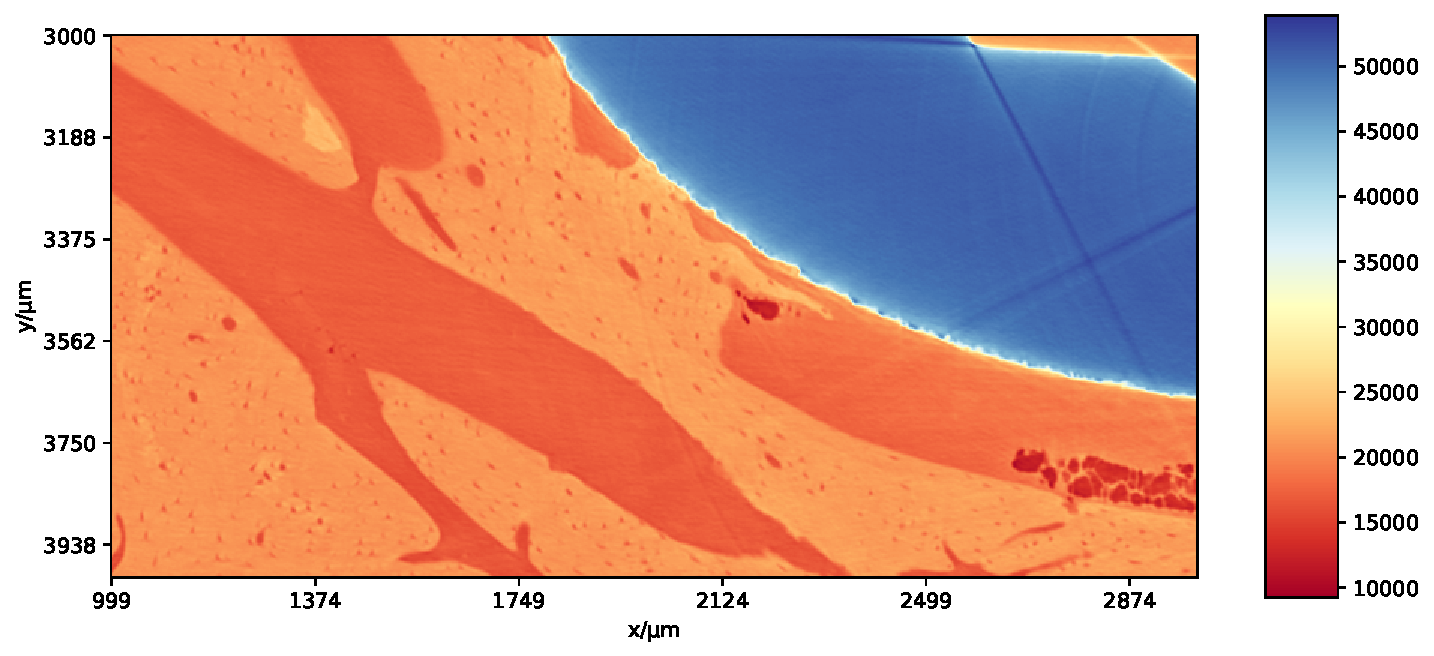
\includegraphics[width=0.85\columnwidth]{generated/770c_pag_roi_yx.pdf}\end{tabular}\\
    \!\!\!\!\!\!(b)\!\!\!&\begin{tabular}{c}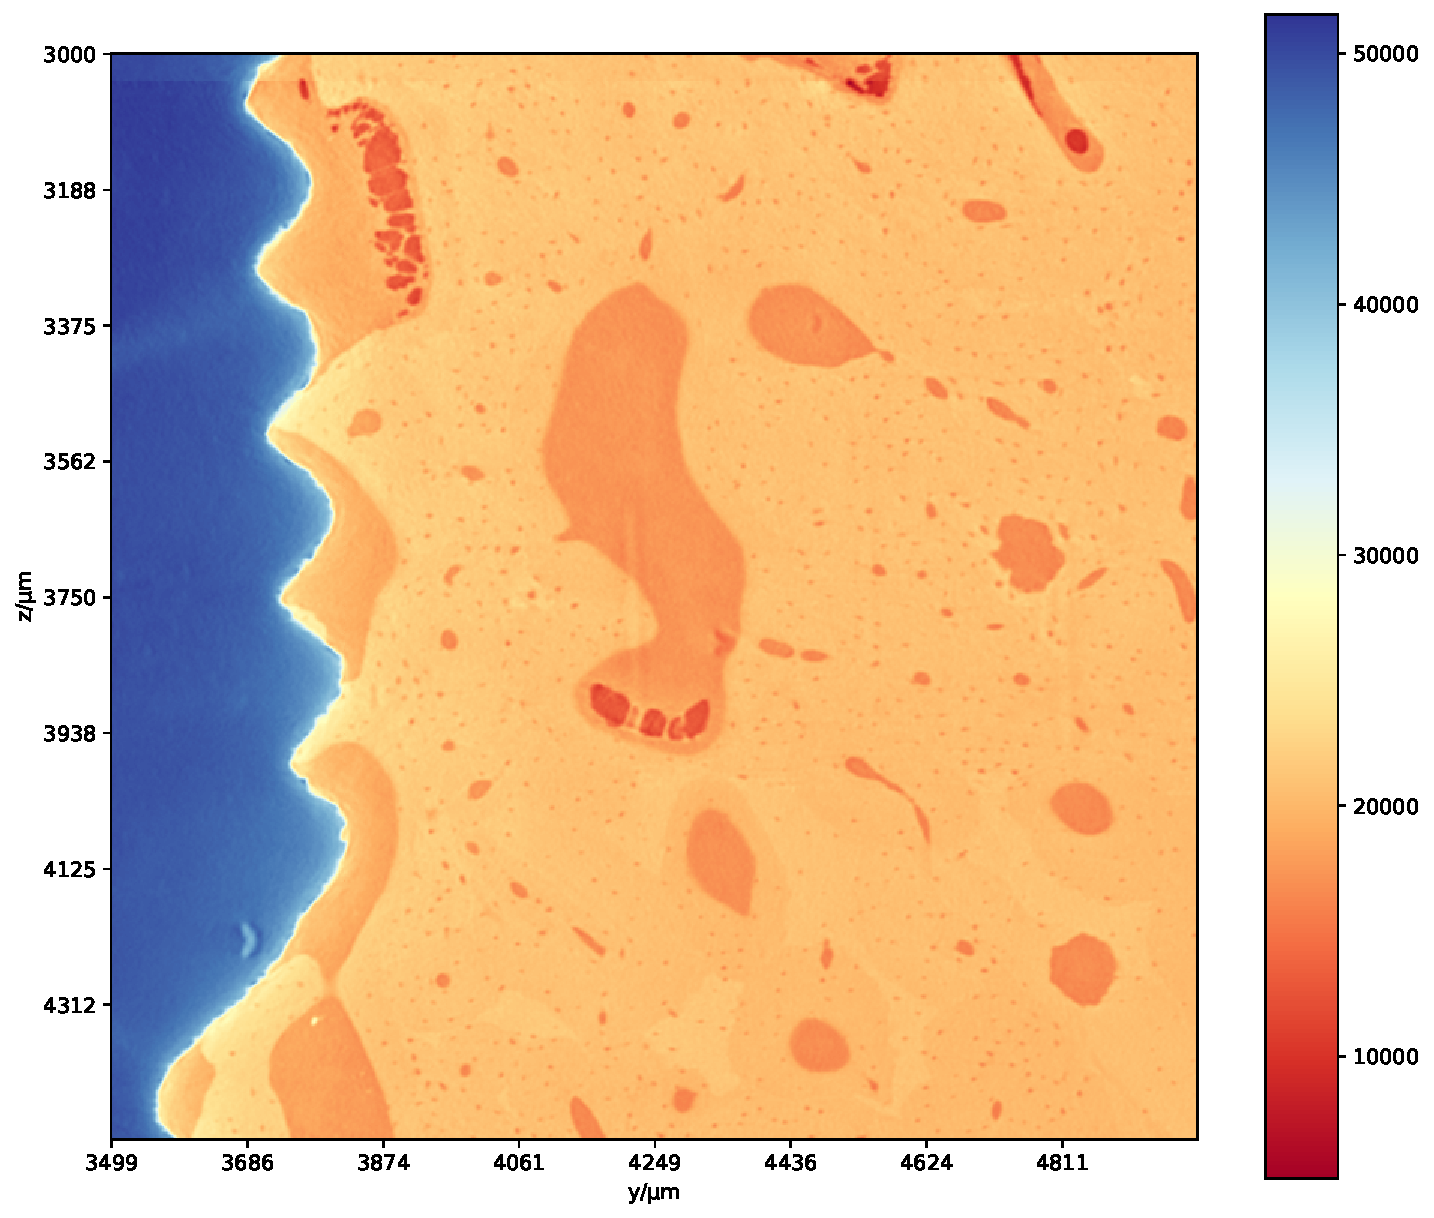
\includegraphics[width=0.85\columnwidth]{generated/770c_pag_roi_zy.pdf}\end{tabular}\\
  \end{tabular}
  \caption{
    To better see the distortion effects, we zoom in on two sub-regions of the
    slices shown in \Cref{fig:3viewsample}. Our visual systems automatically
    correct for most of the distortions, as they appear similar to illumination
    effects. However, even some distance from the implant, blood vessel voxels
    have higher values than bone voxels further out. As we approach the
    implant, the value shifts accelerate and become highly non-linear.
    % TODO highlight this using arrows and absolute values on final images
    (a) A 1 mm $\times$ 2 mm region of an image slice in the YX-plane.
    (b) A 1.5 mm $\times$ 1.5 mm region of an image slice in the ZY-plane in the
    smaller threaded part of the titanium implant.
  }
\label{fig:slices}
\end{figure}

In \Cref{fig:slices}, we see zoomed-in regions of the YX- and ZY-planes of the
same sample as shown in \Cref{fig:3viewsample}. Both planes display a broad
selection of the various types of noise sources found in the data.
% TODO: as other note says... draw/explain in more detail... be specific

We shall go through the main phenomena that result in noise and artifacts
affecting the reconstructed image.

\begin{itemize}
  \item \textbf{Dark and bright streaks:} Streaking artifacts occur close to
	regions with very high absorption, such as metal implants, but also
	to some degree in the transition from dense bone to softer
	tissue.
	This effect is also called photon starvation, due to the
	lowered amount of photons reaching the detector.

	The X-ray beams pass at angles containing
	multiple dense obstacles, the beam is hardened more. Then for
	angles with fewer dense obstacles, the energy spectrum is
	preserved better. This produced the dark and bright streaks
	seen in \Cref{fig:slices}.

	For a hardened beam, softer X-rays are absorbed instead of
	successfully penetrating the object, and will not contribute to
	image formation.  High-density structures such as the titanium
	implant break the isotropy, making the projected X-ray mean
	energy spectrum dependent on incident orientation
	\citep{srnoise}.

	% technically scattering also contributes to this

  \item \textbf{Cupping effect:} A commonly occurring artifact occurs when beams pass
    homogeneous cylindrical objects. Since beams passing the middle will have to
	traverse more material compared to the edges, the beam is hardened more
	towards the center and intensity becomes lower as a result. This can
	manifest itself in what erroneously looks to be dense peripheral
	regions at the edges. A cupping effect also arises from scattering of
	%TODO: xxx want to mention or not?
	which leads to a reduction in low contrast sensetivity

  \item \textbf{Phase contrast:} Phase contrast is used to enhance the contrast
	around soft tissue where the contrast from pure absorption is
	insufficient \citep{phasecontrast}. It can however also induce
	noise, such as fringes around the edges between different
	materials within the sample\citep{srnoise}. Similar to the dark
	and bright streaks artifacts, these effects show up as
	misrepresentations of the voxel values. For the data presented
	here, this is especially prominent at the transitional edges
	between the titanium implant and the biological tissue and
	bone.

  \item \textbf{Ring artifacts:} Looking at the XY-plane in
  	\Cref{fig:slices}(a) we see clear concentric ring artifacts emanating
	from the center of the sample, and at strong edges of the
	titanium implant. It propagates strongly through the large
	region of air behind the implant. This effect arises from
	imperfections in the scanner setup and is typically come from
	uncalibrated or defect adjacent detector elements. For
	synchrotron radiation sources it can also occur from shifts and
	vibrations in the monochromator crystal \citep{ringartefacts}.

  \item \textbf{Projection artifacts:} Bright streaks with strong edges are
	seen from the sharp corners of the titanium implant. When doing back
	projection, sharp corners break the otherwise symmetric
	smearing of projections across the sample.  This can occur from
	the high pass filter used during filtered back projection,
	which exaggerates the differences between adjacent elements
	\citep{ctnoise}.

  \item \textbf{Scattering:} Lower energy rays mostly contribute noise
      from scattering effects. A ray will propagate through a material, get
      scattered and diffract from its initial trajectory. This gives a
      misrepresentation of the attenuation along its initial trajectory. The
      artifacts seen from scattering are similar in nature to those formed by
      beam hardening. This is because both phenomena effectively reduce the
      measured attenuation. For energy levels relevant to the data presented
      here, of 50 keV and above, Compton scattering is the dominant type
      \citep{Compton}. The scattering occurs due to photon-electron interaction
      between the X-ray beam and the material it passes through. Like
      beam-hardening, scattering will cause dark streaks across the image,
      where the attenuation was highest.

      % reference for attenuation values for Ti, Ca, ...
      \citep{attenuation-cross-sections}

      % perhaps rename to scattering in general
      % Ti @ 50 keV
      % photoelectric absorption (dominating), changes contrast due to local absorption within sample of the secondary low energy characteristic x-ray photon.
      % coherent scattering: elastic, not that dominating at 50 keV
      % incoherent scattering: inelastic, adds overall haze/noise and reduces constrast in image, slightly dominates for Ti @ 50 kV, ref

      % The compton scattered x-ray photon can have a significant portion of the energy of the incoming x-ray photon and be measured on the detector as noise.
   \item \textbf{Motion lag:}
   % Well what was the integration time and speed?
   \item \textbf{Partial volume artifacts:}
   %Partial volume artefacts which are dependent on the voxel size and are mentioned briefly by Neldam et al.
\end{itemize}

The distortions that come from the class of physical effects and noise
artifacts discussed in this section, will vary continuously as a function of
the spatial coordinates. This allows the possibility for a method, which can
correctly identify materials despite varying voxel values.

In order for our probability distributions to be suitable for reliable
segmentation,  it is important to ensure that artifacts do in fact have a
continuous imprint.  Since the projections are acquired through rotations using
a very small step size (1/2000 of a degree) then the reconstructed volume can
be assumed to have smoothly/continuously varied features and also artifacts.
Also single projections are assumed to have continuous varying artifacts
because the projections are already heavily denoised, and it is mostly noise
which can be discontinuous.


%%% Local Variables:
%%% mode: latex
%%% TeX-master: "main"
%%% End:
